%!TEX TS-program = xelatex
\documentclass[conference]{IEEEtran}
\usepackage[fontset=founder]{ctex} % 增加中文格式的支持。
%\usepackage[fontset=founder,11pt]{ctex} % 小字体,紧凑一点。
\linespread{1.2}
%\usepackage{cite}
\usepackage[comma, numbers]{natbib}
\usepackage{amsmath,amssymb,amsfonts}
\usepackage{algorithmic}
\usepackage[xetex]{graphicx}
\usepackage{textcomp}
\usepackage{xcolor}
\def\BibTeX{{\rm B\kern-.05em{\sc i\kern-.025em b}\kern-.08em
    T\kern-.1667em\lower.7ex\hbox{E}\kern-.125emX}}

\usepackage[xetex]{hyperref}

\newcommand{\yd}{y^{\text{des}}}
\newcommand{\Yd}{Y^{\text{des}}}
\newcommand{\Ye}{Y^{\text{err}}}
\newcommand{\pd}[2]{\frac{\partial #1}{\partial #2}}
\newcommand{\uff}{u^{\text{ff}}_t}
\newcommand{\fnom}{f_{\text{nom}}}
\newcommand{\ferr}{f_{\text{err}}}
\newcommand{\Var}{\mathrm{Var}}
\DeclareMathOperator{\tr}{tr}
\DeclareMathOperator{\sgn}{sgn}
\newcommand{\Rt}{\mathbb{R}^3}
\newcommand{\R}{\mathbb{R}}


\begin{document}

\title{四旋翼控制的旋转误差度量}

\author{\IEEEauthorblockN{Alexander Spitzer}
\IEEEauthorblockA{\textit{Robotics Institute} \\
\textit{Carnegie Mellon University}\\
Pittsburgh, PA, USA \\
spitzer@cmu.edu}
\and
\IEEEauthorblockN{Nathan Michael}
\IEEEauthorblockA{\textit{Robotics Institute} \\
\textit{Carnegie Mellon University}\\
Pittsburgh, PA, USA \\
nmichael@cmu.edu}
}

\maketitle

\begin{abstract}
  我们分析并实验比较了用于四旋翼控制器的各种旋转误差度量。
  传统的四旋翼姿态控制器使用欧拉角或全旋转来计算姿态误差,并按比例计算控制反应。
  最近,一些研究表明,在姿态控制器中优先考虑四旋翼倾斜,或\textit{推力向量}误差,可以改善位置控制,尤其是在有大的偏航误差的情况下。
  我们提供了一个拟议的旋转度量的目录,将它们放在同一个框架中,并表明我们可以独立地推理和设计反应的量值和反应的方向。
  现有的方法主要分为两类:
    (1) 诱导最短方向的反应以校正全旋转误差的度量,以及 
    (2) 结合最短方向的反应以校正倾斜误差和在最短方向上校正偏航误差的度量。
  %We also show how linearizing the attitude dynamics can improve performance during maneuvers with large yaw error.
  %Finally, we run experiments to compare the various metrics.
  我们展示了实验结果,以突出旋转误差度量之间的显著差异。
  查看 \url{https://alspitz.github.io/roterrormetrics.html} 以交互式模拟形式可视化实验执行。
\end{abstract}


\begin{IEEEkeywords}
  quadrotor, control, nonlinear controls, dynamic inversion, attitude control, rotation representation
\end{IEEEkeywords}

\bstctlcite{IEEEexample:BSTcontrol}

\section{简介}

我们分析和比较了已经提出的用于四旋翼姿态控制器的各种姿态误差度量。

多旋翼飞机最常见的控制结构是级联式的,如图~\ref{fig:control_diag} 所示,其中位置控制器产生一个期望的姿态 $R_{\text{des}}$,然后姿态控制器试图去跟踪它。

\begin{figure}
  \begin{center}
  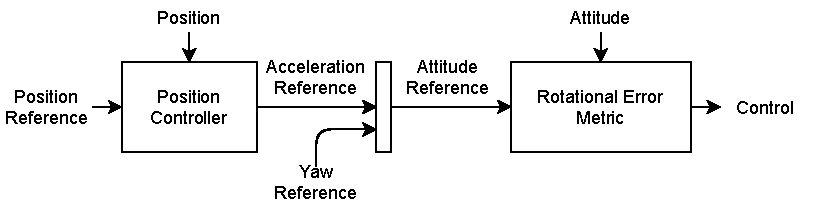
\includegraphics[width=9cm]{media/controllers.pdf}
  \caption{标准的级联四旋翼控制器结构。位置控制器计算出一个期望的加速度,然后将其与偏航参考相结合,为姿态控制器生成一个姿态参考。姿态控制器然后使用旋转误差度量来计算控制。}
  \label{fig:control_diag}
  \end{center}
\end{figure}

为简洁起见,我们考虑的是规则,而不是轨迹跟踪,但这里的所有结果都可以扩展为适用于轨迹跟踪,其中期望的角速度 $\omega_{\text{des}}$ 和期望的角加速度 $\alpha_{\text{des}}$ 均为非零。

我们考虑的四旋翼姿态控制器的结构是旋转误差PD控制器,由旋转误差度量 $e_R$ 和角速度 $\omega$ 定义,前者由对角的姿态增益矩阵 $K_R$ 缩放,后者由对角的角速度增益矩阵 $K_\omega$ 缩放。

\newcommand{\Rdes}{R_{\text{des}}}
\newcommand{\zdes}{z_{\text{des}}}

\begin{align}
  \alpha = -K_R e_R(R, \Rdes) - K_\omega \omega
\end{align}

参考文献中的几项工作已经指出,由于四旋翼的位置动力学仅取决于其倾斜度,或机体 $z$ 轴,因此将飞行器的倾斜优先于飞行器的偏航是有意义的 [\citenum{brescianini_nonlinear_2013,faessler_automatic_2015,mueller_multicopter_2018,kooijman_trajectory_2019,gamagedara_geometric_2019}]。
在本项工作中,我们证实了这一点,并表明这种度量相当于在当前和期望的机体 $z$ 轴之间的交叉乘积方向上诱发反应,以及围绕机体 $z$ 轴的反应。
我们表明,这种分解比使用全旋转误差的传统姿态控制器更好地线性化了车辆误差反应。
在存在大的跟踪误差的情况下,遵循直线路径对整体控制性能是有利的。

%We also show a feedback linearization addition to attitude controllers that improves performance during maneuvers with large yaw error.

\section{旋转误差度量}

\subsection{预备知识}

在本节中,我们将文献中所使用的各种控制器放置在上面所描述的框架中。
首先,在文献 \citet{mueller_multicopter_2018} 中,我们将旋转误差 $R_e$ 定义为 

\begin{align}
  R_e = \Rdes^\top R
\end{align}
并且其相应的角度和轴为 $\rho_e$ 和 $n_e$。

飞行器姿态 $R$ 将向量从机体帧 $\mathcal B$ 变换到固定帧中,并用一个矩阵表示,其列 $x$、$y$ 和 $z$ 是机体的坐标帧的轴。

\begin{align}
  R = \begin{pmatrix} x & y & z \end{pmatrix}
\end{align}

我们将\textit{推力向量}误差 $R_{tv}$ 定义为当前和期望姿态的 $z$ 轴之间的旋转,以及与其相关的角度 $\rho_{tv}$ 和轴 $n_{tv}$。
该旋转可以通过其角度和轴定义为全旋转误差 $R_e$,展示在文献 \citep{mueller_multicopter_2018} 中。

\begin{align}
  \rho_{tv} &= \cos^{-1}(e_3^\top R_e e_3) \\
  n_{tv} &= \frac{(R_e^\top e_3) \times e_3 }{|| (R_e^\top e_3) \times e_3 || }
\end{align}

为帮助理解 $n_{tv}$,请注意它只是期望的$z$轴 $\zdes^{\mathcal{B}} = R^\top\Rdes e_3$ 与当前机体的$z$轴 $z^{\mathcal{B}} = e_3$ 的归一化叉乘,在机体帧中表示。
作为结果,$n_{tv}^\top e_3 = 0$。

\begin{align}
  n_{tv} = \frac{
                  \zdes^{\mathcal{B}} \times z^{\mathcal{B}}
                }
                { ||
                  \zdes^{\mathcal{B}} \times z^{\mathcal{B}}
                || }
\end{align}

我们将偏航误差 $R_{\text{yaw}}$ 定义为围绕机体 $z$ 轴的剩余误差,即在对齐 $z$ 轴后,将当前旋转与期望旋转对齐所需的旋转。

\begin{align}
  R_{\text{yaw}} = R_e R_{tv}^{-1}
\end{align}

$\rho_{\text{yaw}}$ 表示与 $R_{\text{yaw}}$ 相关的角度,并且 $n_{\text{yaw}}$ 表示轴,它要么是 $e_3 = (0, 0, 1)^\top$ 或者是 $-e_3$,并因此与 $n_{tv}$ 垂直。
\subsection{全旋转度量}

在文献 [\citenum{lee_geometric_2010,mellinger_minimum_2011,goodarzi_geometric_2013}] 中使用了直接以 $SO(3)$ 表示的旋转误差度量。
如文献 \cite{mueller_multicopter_2018} 所示,该度量与角度误差 $\rho_e$ 的正弦成比例,并在最短路径 $n_e$ 的方向上。

\begin{align}
  \label{eq:skew}
  e_R^{\textbf{A}}(R, \Rdes) = \frac12\left(R_e - R_e^\top\right)^\vee = \sin\rho_e n_e
\end{align}

在文献 \citet{lee_exponential_2012} 中指出使用与误差正弦成比例的旋转误差度量的问题,即当误差为 $90^\circ$ 时,反应最强,而当误差再增大时,反应减弱,当误差为 $180^\circ$ 时,反应为零。 
虽然这确保了反应的平滑性,但当误差较大时,其结果会导致收敛缓慢。
在文献 \citet{lee_exponential_2012} 中提议重新调整旋转误差的比例。 \footnote{我们添加了一个 $2$ 的因子以匹配方程 \eqref{eq:skew} 围绕 $\rho_e = 0$ 的线性化。}

\begin{align}
  \label{eq:scaled_skew}
  e_R^{\textbf{B}}(R, \Rdes) = \frac{2}{\sqrt{1 + \tr\left(R_e\right)}}\sin\rho_e n_e
\end{align}

使用 $\tr\left(R_e\right) = 2\cos\rho_e + 1$ \citep{mueller_multicopter_2018} 和正弦半角特性 $\sin\left(\frac{\theta}{2}\right) = \sqrt{\frac{1 - \cos\theta}{2}}$ 的事实,
方程 \eqref{eq:scaled_skew} 可被重写为

\begin{align}
  \label{eq:sinhalf_full}
  e_R^{\textbf{B}}(R, \Rdes) = 2\sin\left(\frac{\rho_e}{2}\right) n_e.
\end{align}

方程 \eqref{eq:sinhalf_full} 在数学上等同于在文献 \citet{fresk_full_2013} 中使用的旋转误差,它是误差四元数的轴分量。四元数的轴分量是半角的正弦值乘以轴。

同样地,可以使用与角度成比例的误差反应。

\begin{align}
  \label{eq:angle_full}
  e_R^{\textbf{C}}(R, \Rdes) = \rho_e n_e.
\end{align}

这可能没有被广泛应用,因为与方程 \eqref{eq:skew} 和方程 \eqref{eq:scaled_skew} 不同,从旋转矩阵或四元数姿态表示中评估方程 \eqref{eq:angle_full} 需要反三角函数评估,这在嵌入式平台上可能很昂贵。

\subsection{推力向量 -- 偏航分解度量}

在本节中,我们将刻画工作中所使用的姿态控制,它们将姿态分解为推力向量和偏航,被称为``减小姿态控制'',其重点是围绕机体 $x$ 和 $y$ 轴的控制。
定义,$\omega_{XY} = z \times \dot z = \omega - \left(\omega^\top z\right) z$。

在文献 \citet{kooijman_trajectory_2019} 中将姿态表示分解为 $\mathcal S_2 \times \mathcal S_1$,这相当于控制推力向量方向,即一个 $\mathcal S_2$ 的元素,独立于围绕推力向量的旋转,即一个 $\mathcal S_1$ 的元素。
围绕 $x$ 和 $y$ 轴\footnote{为简单起见,我们省略在文献 \citet{kooijman_trajectory_2019} 中的偏航控制器。}的控制反应,在文献 \citet{kooijman_trajectory_2019} 中给出为 

\begin{align}
  \label{eq:s2s1_omxy}
  \omega_{XY}^{\mathcal B} &= R^\top ( z \times u_v ) \\
              &= e_3 \times (R^\top u_v) \\
              &= \begin{pmatrix} -y^\top u_v \quad x^\top u_v \quad 0 \end{pmatrix}^\top,
\end{align}

其中 $u_v$ 定义为

\begin{align}
  \label{eq:uvdef}
  u_v =
    \begin{cases}
    k_1 \zdes &  \rho_{tv} \leq \frac\pi2 \\
    \frac{k_1}{\sqrt{1 - (z^\top\zdes)^2}} \zdes =
    \frac{k_1}{\sin\rho_{tv}} \zdes &  \frac\pi2 < \rho_{tv} < \pi.
  \end{cases}
\end{align}

将 \eqref{eq:uvdef} 代入 \eqref{eq:s2s1_omxy},我们得到 

\begin{align}
  \label{eq:s2s1_omxy2}
  \omega_{XY}^{\mathcal B} =
  \begin{cases}
    -k_1 \zdes^{\mathcal B} \times z^{\mathcal B} = -k_1 \sin\rho_{tv} n_{tv} &  \rho_{tv} \leq \frac\pi2 \\
    -k_1 \frac{\zdes^{\mathcal B} \times z^{\mathcal B}}{\sin\rho_{tv}} = -k_1 n_{tv} & \frac\pi2 < \rho_{tv} < \pi.
  \end{cases}
\end{align}

假设对于角速度为 P 控制器,从方程 \eqref{eq:s2s1_omxy2} 中,我们可以提取旋转误差度量 $e_R$ 为 

\begin{align}
  \label{eq:s2s1_re}
  e_R^{\textbf{D}}(R, \Rdes) =
   \begin{cases}
     \sin\rho_{tv} n_{tv} & \rho_{tv} \leq \frac\pi2 \\
     n_{tv} & \frac\pi2 < \rho_{tv} < \pi.
   \end{cases}
\end{align}

方程 \eqref{eq:s2s1_re} 有一个有趣的特性,即反应的量值在 $\rho_{tv} = \frac\pi2$ 的角度处是最大的,并且随着角度从 $\frac\pi2$ 增加到 $\pi$ 时保持不变。 
对于 $\rho_{tv} \leq \frac\pi2$,方程 \eqref{eq:s2s1_re} 等同于方程 \eqref{eq:skew} 的轴对齐误差。

在文献 \citet{brescianini_tilt-prioritized_2020} 中也分解推力向量和偏航,但使用了两个四元数。
最终的控制法是以四元数误差表示的推力方向误差和以四元数误差表示的围绕机体 $z$ 轴的角度误差之和。
四元数的使用意味着旋转误差的度量与推力向量误差和偏航误差的半角正弦成比例。
由此产生的旋转误差度量如下所示,并再次添加了 $2$ 的系数,以匹配与其他度量的线性化。

\begin{align}
  \label{eq:quat_decomp}
  e_R^{\textbf{E}}(R, \Rdes) = 2\sin\left(\frac{\rho_{tv}}{2}\right) n_{tv} + 2 \sin\left(\frac{\rho_{\text{yaw}}}{2}\right) n_{\text{yaw}}
\end{align}

对于轴对齐的误差,方程 \eqref{eq:quat_decomp} 等同于方程 \eqref{eq:sinhalf_full}。

在文献 \citet{mueller_multicopter_2018} 中提出了一种新的旋转误差度量,它有效地在方程 \eqref{eq:angle_full} 和仅控制推力向量之间进行线性插值。旋转误差度量如下所示,在 $\alpha_{\text{yaw}} \in [0, 1]$ 区间对偏航角的控制使用加权。

\begin{align}
  \label{eq:mueller4}
  e_R^{\textbf{F}}(R, \Rdes) = \alpha_{\text{yaw}} \rho_e n_e + (1 - \alpha_{\text{yaw}}) \rho_{tv} n_{tv}
\end{align}

与方程 \eqref{eq:s2s1_re} 和方程 \eqref{eq:quat_decomp} 不同,对于 $\alpha_{\text{yaw}} > 0$,方程 \eqref{eq:mueller4} 不会将偏航控制与推力向量控制解耦。
正如我们将在下面显示的那样,在某些大的角度误差情况下,这导致了次优的性能。
作为一个替代,我们提议使用来自方程 \eqref{eq:quat_decomp} 的解耦度量,但与角度成比例,如下所示。

\begin{align}
  \label{eq:propose1}
  e_R^{\textbf{G}}(R, \Rdes) = \rho_{tv} n_{tv} + \rho_{\text{yaw}} n_{\text{yaw}}
\end{align}

\begin{table}
  \begin{center}
  \caption{Comparison matrix of various rotational error metrics}
  \label{tab:comp}
  \begin{minipage}{\textwidth}
  \begin{tabular}{c|c|c}
    \textbf{Scaling / Direction} & \textbf{Full}: $n_e$ & \textbf{Decomposed}: $n_{tv} + n_{\text{yaw}}$ \\ \hline
    $\sin\rho$ &
      $e_R^{\textbf{A}}$: [\citenum{lee_geometric_2010,mellinger_minimum_2011,goodarzi_geometric_2013}] &
      $e_R^{\textbf{D}}$\footnote{For $\rho < \frac\pi2$.}: [\citenum{kooijman_trajectory_2019,gamagedara_geometric_2019}]
    \\ \\[-2.0mm] \hline \\[-2.8mm]
    $2\sin\frac\rho2$ &
      $e_R^{\textbf{B}}$: [\citenum{lee_exponential_2012,fresk_full_2013}] &
      $e_R^{\textbf{E}}$: [\citenum{brescianini_nonlinear_2013,faessler_automatic_2015,mueller_multicopter_2018,brescianini_tilt-prioritized_2020}]
    \\ \\[-2.0mm] \hline \\[-2.8mm]
    $\rho$ &
    $e_R^{\textbf{C}}$, $e_R^{\textbf{F}}$\footnote{For $\alpha_{\text{yaw}} > 0$.}: [\citenum{mueller_multicopter_2018}] &
      $e_R^{\textbf{G}}$: Proposed
  \end{tabular}
  \end{minipage}
  \end{center}
\end{table}


表~\ref{tab:comp} 提供了所讨论的旋转误差度量配置的列表摘要。

%\input{fblin}

\section{实验}

为了评估用于四旋翼控制的旋转误差度量,我们使用了以下三种情况。

\begin{enumerate}
  \item 方向改变。
  \item 具有大的初始偏航误差的轴对齐步骤。
  \item 对角线步骤。
\end{enumerate}

在最后两个实验中,我们还与基于欧拉角的旋转误差度量进行了比较,该度量是使用 Z-Y-X 约定定义的。
偏航 $\psi$、俯仰 $\theta$ 和横滚 $\phi$ 使用以下映射 $F(\psi, \theta, \phi)$ 定义旋转矩阵,其中 $c = \cos$ 并且 $s = \sin$。

\begin{align}
  F = \begin{pmatrix} c\psi c\theta & c\psi s\theta s\phi - c\phi s\psi & s\psi s \phi + c\psi c\phi s\theta \\
  c\theta s\psi & c\psi c\phi + s\psi s\theta s\phi & c\phi s\psi s\theta - c\psi s\phi \\
-s\theta & c\theta s\phi & c\theta c\phi \end{pmatrix}
\end{align}

然后使用 $F$ 的逆矩阵定义旋转误差度量,确保计算每个角度的最短角距离。

\begin{align}
  e_R^{\textbf{ZYX}}(R, \Rdes) = F^{-1}(R) \ominus F^{-1}(\Rdes)
\end{align}

\subsection{方向改变}

四旋翼飞机的任务是在原点以 $(0, -5, 0)$ 的速度和 $80^\circ$ 的初始横滚角开始后到达 $(0, 3, 0)$ 的目标位置。
这个初始条件被设计为诱导大于 $90^\circ$ 的初始横滚误差,以便突出大的角度误差下旋转误差度量反应的差异。

\begin{figure}
  \begin{center}
  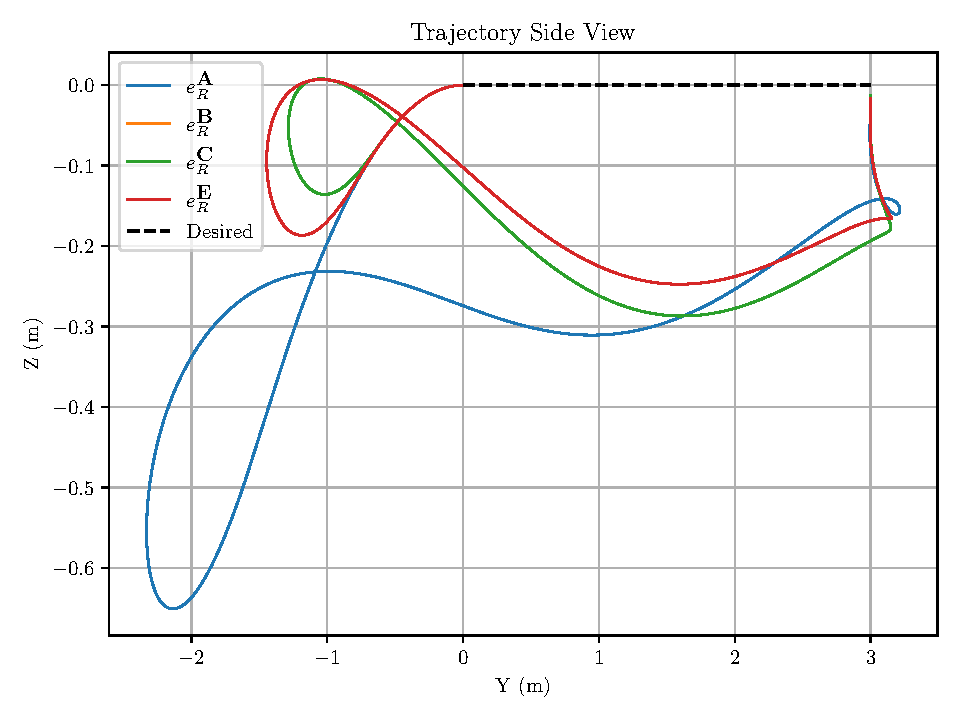
\includegraphics[width=8cm]{media/quickchange/sideview.pdf}
  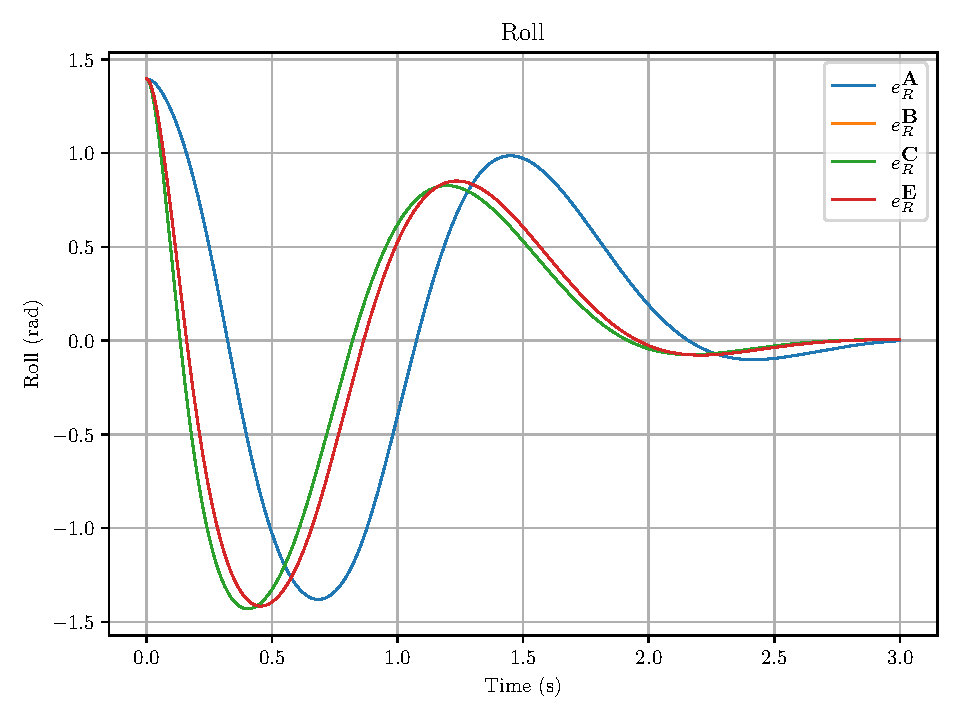
\includegraphics[width=8cm]{media/quickchange/Roll.pdf}
  \caption{在各种旋转误差度量的快速方向改变测试期间,跟踪轨迹(顶部)和横滚(底部)的侧视图。与角度正弦成比例的反应的度量,\textbf{A},其收敛速度远慢于与半角正弦,\textbf{B} 和 \textbf{E},或与角度,\textbf{C},成比例的反应的度量。由于轨迹位于 $YZ$ 平面中,\textbf{B} 和 \textbf{E} 执行相同的操作。}
  \label{fig:qc_side}
  \end{center}
\end{figure}

图~\ref{fig:qc_side} 显示了产生的侧视图和横滚轨迹。
这里需要注意的重要一点是,旋转误差度量 $e_R^{\textbf{A}}$,其反应与角度误差的正弦成比例,收敛速度比其它度量更慢。
该示例表明,当存在大的姿态误差时,导致反应与角度正弦成比例的度量可能会出现缓慢收敛。

\subsection{带有偏航误差的步骤}

在这个测试中,四旋翼飞机同时执行位置步骤和偏航步骤。
飞行器从原点开始,偏航角为 $90^\circ$,并以 $0^\circ$ 的偏航角移动到 $(0, 3, 0)$。

\begin{figure}
  \begin{center}
  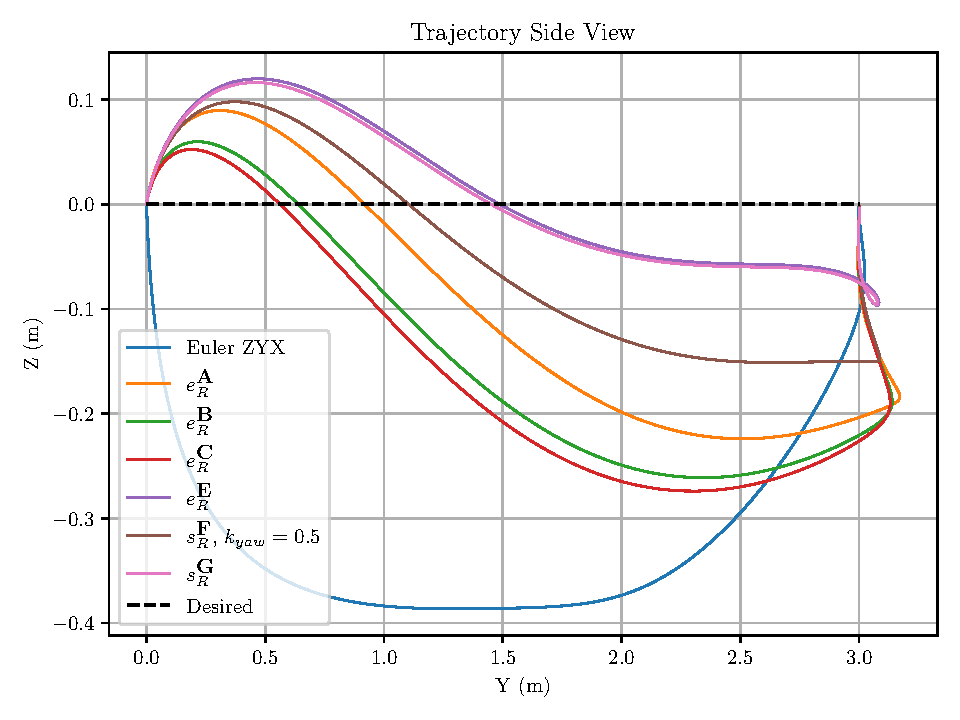
\includegraphics[width=8cm]{media/yawstep/sideview.pdf}
  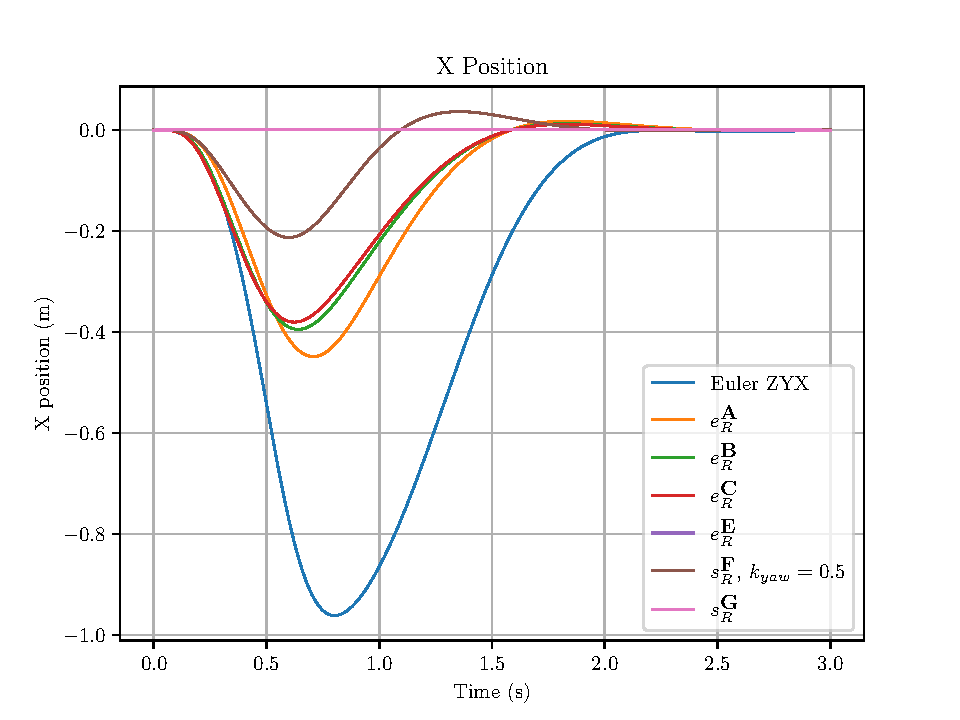
\includegraphics[width=8cm]{media/yawstep/X_Position.pdf}
  \caption{各种旋转误差度量下,在同时进行 $3$ m 位置步骤和 $90^\circ$ 偏航步骤期间,跟踪轨迹(顶部)和 $x$ 位置(底部)的侧视图。只有将推力向量从偏航中分解出来的度量,\textbf{E} 和 \textbf{G},才能保持期望的 $x$ 位置。}
  \label{fig:ys_side}
  \end{center}
\end{figure}

图~\ref{fig:ys_side} 显示了实验期间的侧视图和 $x$ 位置。
我们看到,使用全旋转误差的度量,导致轨迹不能保持期望的 $x$ 位置。
分解反应的度量,\textbf{E} 和 \textbf{G},保持了期望的 $x$ 位置。

\subsection{对角线步骤}

在这个测试中,我们表明,对于旋转误差度量,偏航误差不是必需的,因为旋转误差度量不会将推力矢量与偏航解耦,从而表现出次优性能。
四旋翼飞机被赋予一个从原点到 $(3, 3, 0)$ 的对角线步骤,在测试期间,期望的偏航为 $0^\circ$。

\begin{figure}
  \begin{center}
  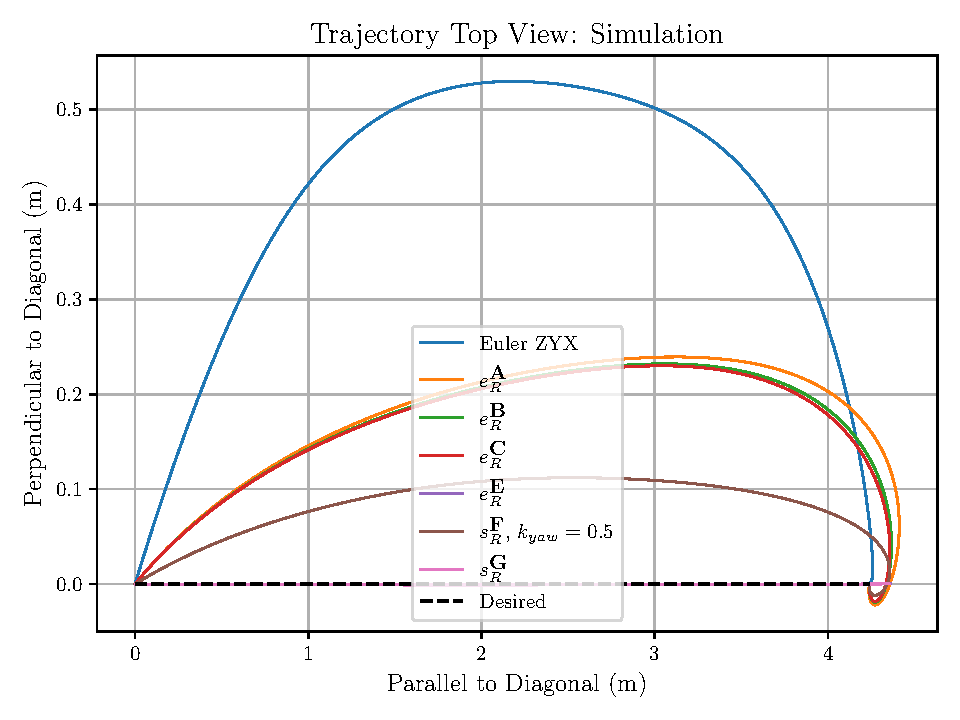
\includegraphics[width=8cm]{media/diagstep/topview.pdf}
  \caption{在从原点到 $(3, 3, 0)$ 的对角线步骤中,各种旋转误差度量的轨迹俯视图。只有将推力向量从偏航中分解出来的度量,\textbf{E} 和 \textbf{G},保持在直线的对角线路径上。}
  \label{fig:ds_top}
  \end{center}
\end{figure}

图~\ref{fig:ds_top} 显示了各种误差度量的实验过程中跟踪轨迹的俯视图。
使用全旋转误差的度量,\textbf{A},\textbf{B},\textbf{C} 和 \textbf{F},偏离了对角线路径。
这是因为在 $SO(3)$ 中,从幺元到导致飞行器以相同的偏航角的对角加速的最短路径,需要飞行器通过在对角以外的方向的加速方向。换句话说,投射到水平面上的推力向量并不指向期望位置的方向。

将误差分解为推力向量分量和偏航分量的度量,\textbf{E} 和 \textbf{G},沿着直线的对角线路径到达期望位置。


\section{讨论}

我们已经证明,文献中的许多四旋翼姿态控制器可以使用其旋转误差度量的缩放和方向来整齐地刻画。

我们已经证明,将姿态误差分解为推力向量分量和偏航分量的旋转误差度量,比那些使用全姿态误差的旋转误差度量,在 (1) 位置和偏航同时存在大的误差,以及 (2) 对角线步骤时,提供了更优的控制性能。


%We model the quadrotor as a rigid body, with the addition of unknown, but deterministic, acceleration and angular acceleration disturbances.
%
%The state and control vectors are shown below.
%
%\begin{equation}
%  \mathbf x = \begin{pmatrix} p \\ v \\ R \\ \omega \end{pmatrix}\quad
%  \mathbf u = \begin{pmatrix} u \\ \alpha \end{pmatrix}
%\end{equation}
%
%Here, $p \in \Rt$, $v \in \Rt$, $R = \begin{bmatrix} x & y & z \end{bmatrix} \in SO(3)$, $\omega \in \Rt$ represent the vehicle position, velocity, attitude, and angular velocity, while $u \in \R$ and $\alpha \in \Rt$ represent the thrust along the body $z$-axis, $z$, and body angular acceleration.
%$R$ represents the transformation from the body frame to the world frame, $p$ and $v$ are expressed in the world frame, and $\omega$ and $\alpha$ are expressed in the body frame.
%
%The dynamics are shown below.
%
%\begin{align}
%  \dot p &= v \\
%  \dot v &= uz + g + a_e(\mathbf x) \\
%  \dot R &= R [ \omega ]_\times \\
%  \dot \omega &= \alpha + \alpha_e(\mathbf x)
%\end{align}
%
%Here, $g$ is the gravity vector, $a_e(\mathbf x)$ is the additive linear acceleration disturbance, and $\alpha_e(\mathbf x)$ is the additive angular acceleration disturbance.

\bibliographystyle{IEEEtranN}
\bibliography{IEEEabrv,refs}

\end{document}
